\subsection{Architecture générale}

Le transformeur a une architecture encodeur--décodeur.
L'encodeur est composé d'une couche de plongement positionnel 
suivi d'une couche d'auto-attention et d'un \gls{mlp}.
Le décodeur est identique mais ajoute une couche d'attention croisée entre les deux . 
Chacune des couches susmentionnées est suivie d'une couche de normalisation~\cite{Ba_Kiros_Hinton_2016}
avec une connexion résiduelle (Voire Figure~\ref{fig.transformer}).

\begin{figure}[htb]
    \centering
    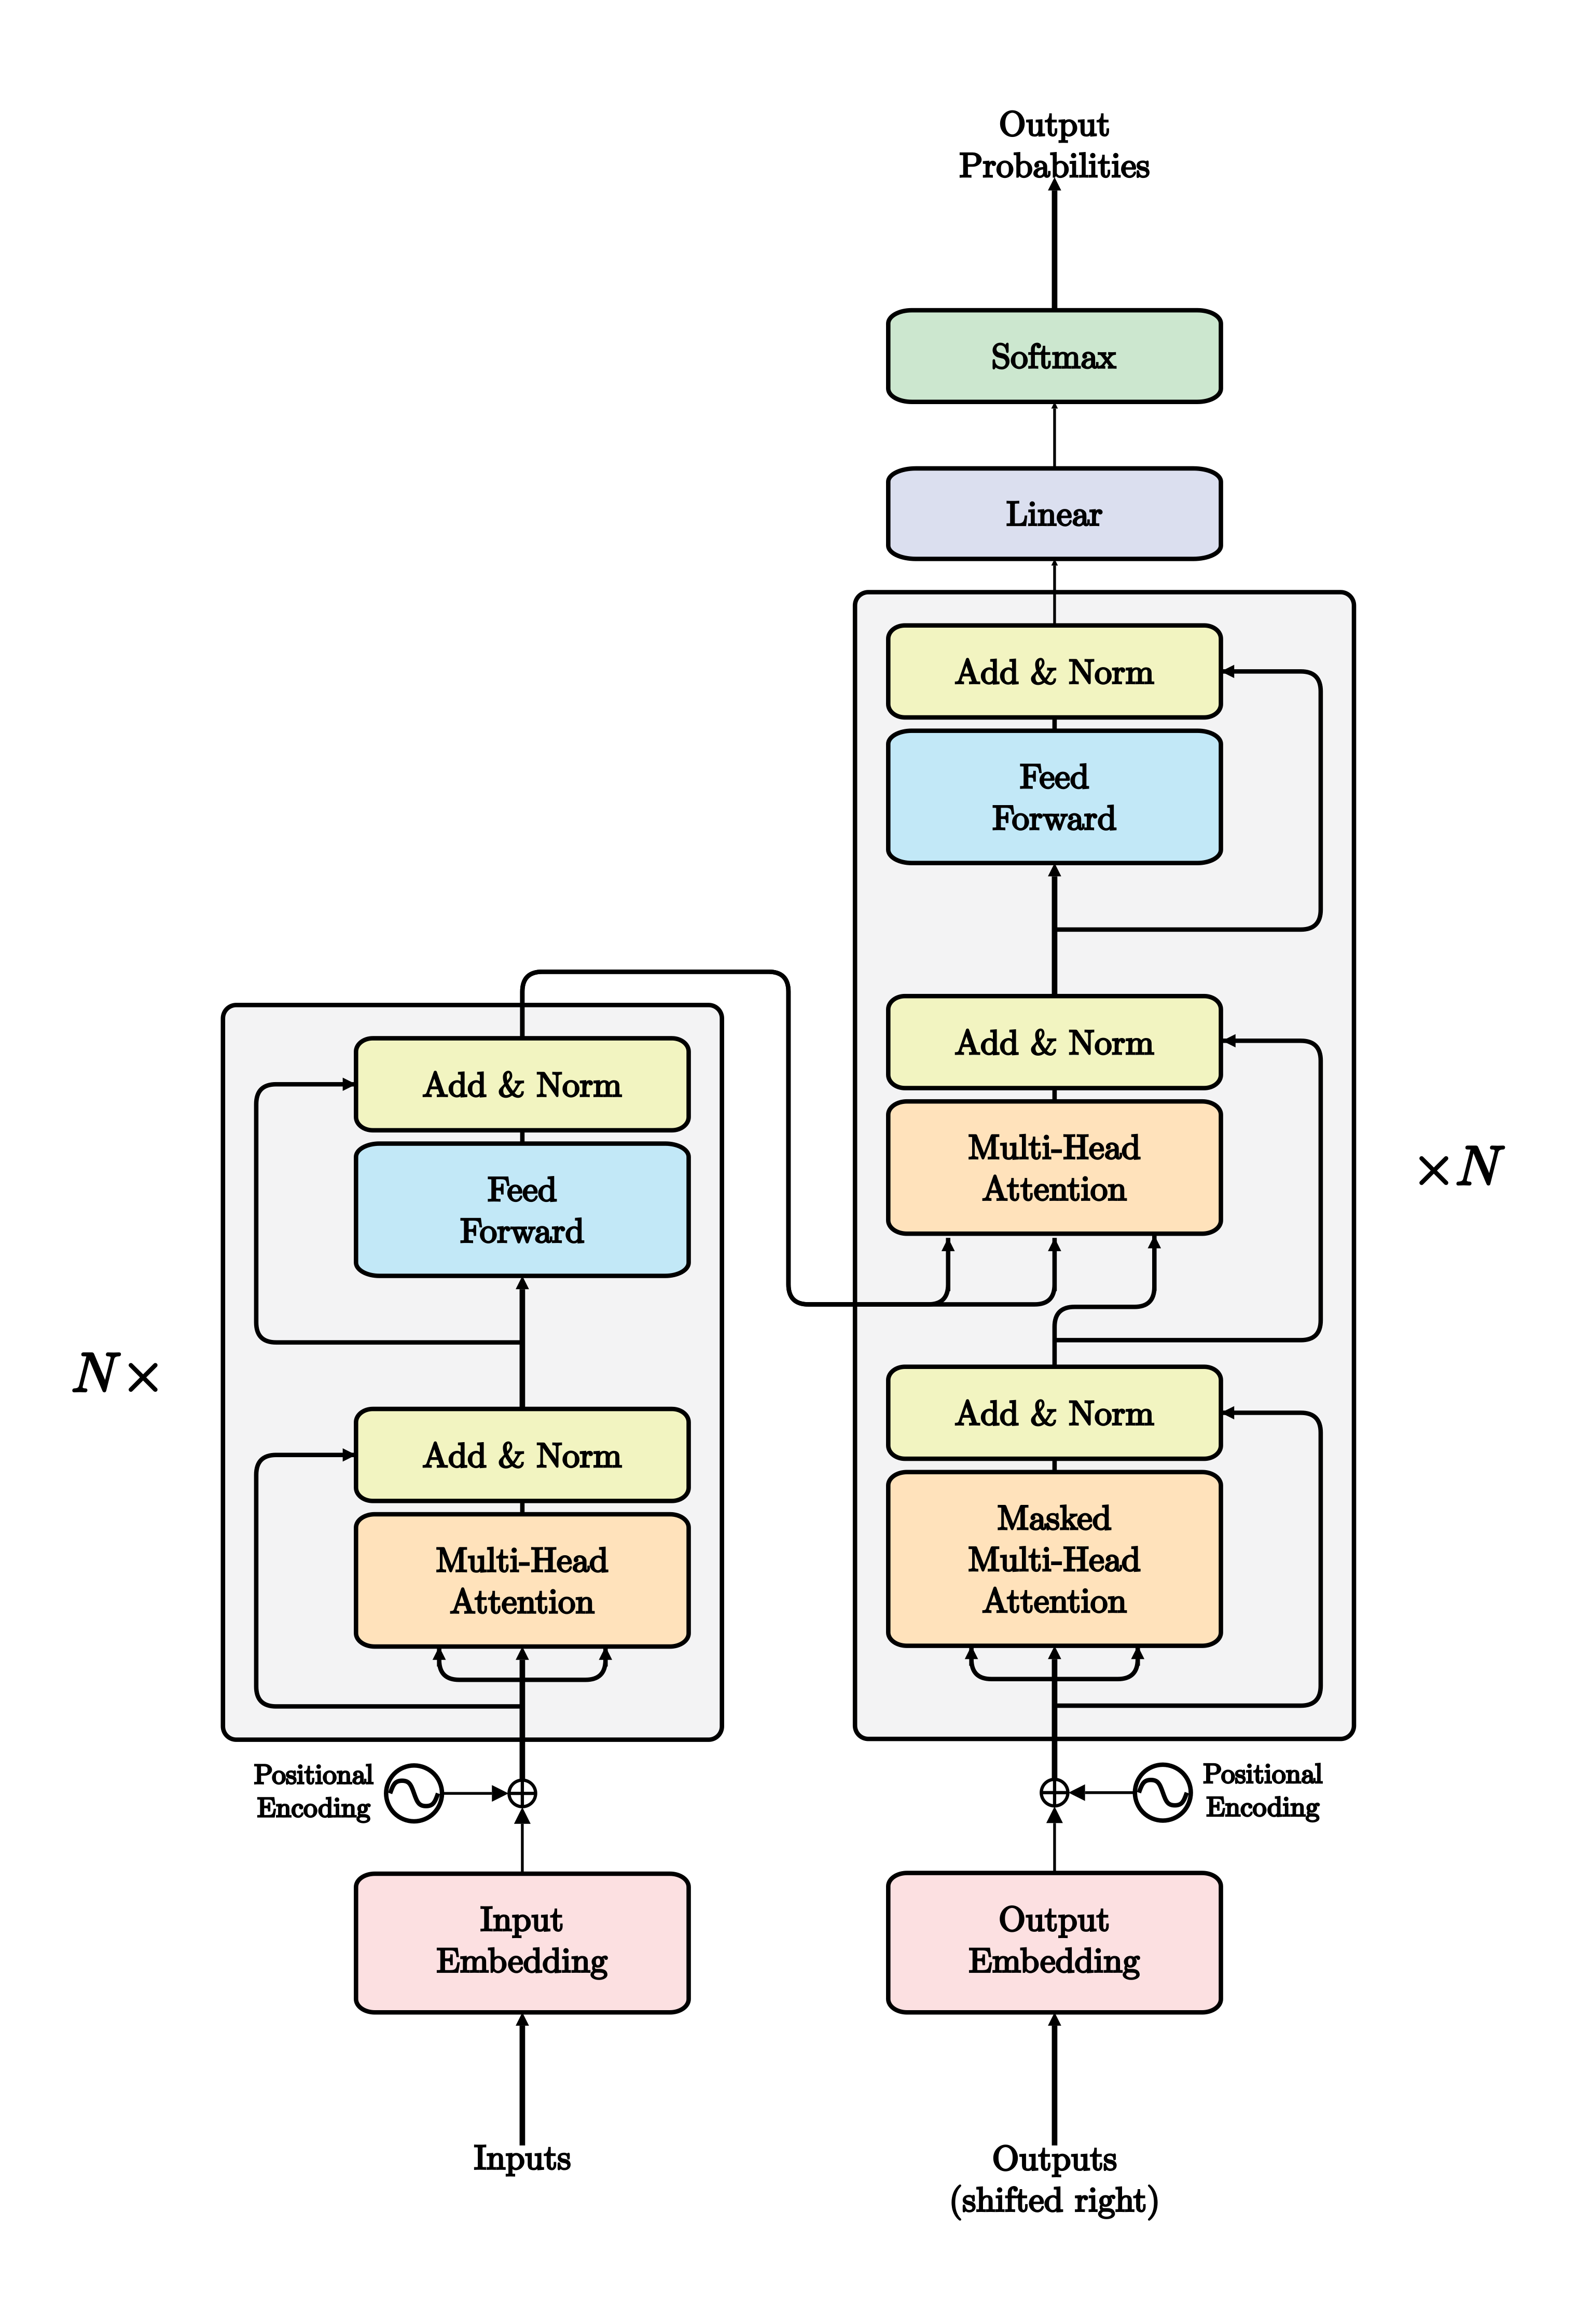
\includegraphics[width=8cm]{assets/images/transformer.png}
    \caption[L'architecture de transformeur.]%
    {L'architecture de transformeur~\cite[Fig 1]{attention}.}
    \label{fig.transformer}
\end{figure}
